Consider an implicit (closed) curve in 2D

$$
f(x, y) = 0
$$

given by a particular parameterization $x = x(t)$, $y = y(t)$, where $t \in [0, L]$. For a choice of parameter values
$\{t_j\} = \{t_1, \dots, t_N\}$, consider the point cloud 
$\{ \bm{x}_j = \left( x_j, y_j \right) = \left( x_j(t), y_j(t) \right) \}$. Suppose we wish to reconstruct the implicit 
function from the given point cloud.


\begin{enumerate}[(i)]
  \item $(x_k)_{k \in \mathbb{N}}$, where $x_k = 2^{-k}$.

\begin{solution}
  Let $C > 1$ for any $C \in \mathbb{R}$. Then we have

  $$
  \frac{C^{-(k+1)}}{C^{-k}} = \frac{C^k}{C^{k+1}} = \frac{1}{C} < 1
  $$

  and so the sequence $(a_k)$ defined by $a_k = C^{-k}$ converges by the Ratio Test. Moreover, for any $\epsilon > 0$,
  we may choose sufficiently large $N \in \mathbb{N}$ such that $\left|\frac{1}{C^{k}} - 0 \right| < \epsilon$ whenever 
  $k > N$ and so (with $C = 2$) $\lim\limits_{k \to \infty} a_k = 0$. Hence (for $C = 2$) 
  $\Vert e_{k} \Vert = \frac{1}{2^k}$ and so we find

  $$
    \lim\limits_{k \to \infty} \frac{\Vert e_{k+1} \Vert}{\Vert e_k \Vert^1} 
        = \lim\limits_{k \to \infty} \frac{2^{-(k+1)}}{2^{-k}} \\
        = \lim\limits_{k \to \infty} \frac{2^k}{2 \cdot 2^k} \\
        = \frac{1}{2}.
  $$

  The rate of convergence of $(x_k)$ is therefore $r = 1$ with rate constant $C = \frac{1}{2}$ and so the convergence
  of $(x_k)$ is linear.
  \ \\
\end{solution}
  \pagebreak
  \item $(x_k)_{k \in \mathbb{N}}$, where $x_k = 1 + 5 \left(10^{-2k}\right)$.

\begin{solution}
  Observe that each $x_k$ is bounded below by 1.
  Let $C > 1$ for any $C \in \mathbb{R}$. The difference between each successive term in the sequence is given by

  \begin{align*}
    x_{k+1} - x_{k} &= 5 \cdot 10^{-2(k+1)} - 5 \cdot 10^{-2k} \\
                    &= 5 \cdot 100^{-(k+1)} - 5 \cdot 100^{-k} \\
                    &= 5 \cdot 100^{-k} \left( \frac{1}{100} - 1 \right) \\
                    &< 0.
  \end{align*}

  The sequence $(x_k)$ is therefore monotonically decreasing and bounded below, and hence it converges. Moreover, the 
  limit of the sequence is given by

  $$
  \lim\limits_{k \to \infty} 1 + 5\left( 10^{-2k} \right)
      = 1 + 5 \cdot \lim\limits_{k \to \infty} \left( \frac{1}{100^k} \right)
      = 1
  $$

  by (i). We therefore observe that $\Vert e_{k} \Vert = 5 \cdot 100^{-k}$ and so we find

  $$
    \lim\limits_{k \to \infty} \frac{\Vert e_{k+1} \Vert}{\Vert e_k \Vert^1} 
        = \lim\limits_{k \to \infty} \frac{5 \cdot 100^{-(k+1)}}{5 \cdot 100^{-k}} \\
        = \lim\limits_{k \to \infty} \frac{100^k}{100 \cdot 100^k} \\
        = \frac{1}{100}.
  $$

  The rate of convergence of $(x_k)$ is therefore $r = 1$ with rate constant $C = \frac{1}{100}$ and so the convergence
  of $(x_k)$ is linear.
  \ \\
\end{solution}
  \pagebreak
  \item \begin{mini*}
  {}{z = x_1 - 2x_2}{}{}
  \addConstraint{x_1 - 2x_2}{\geq 4}
  \addConstraint{x_1 + x_2}{\leq 8}
  \addConstraint{x_1, x_2}{\geq 0}.
\end{mini*}


\begin{solution}
  \ \\
  \begin{figure}[h]
    \centering
    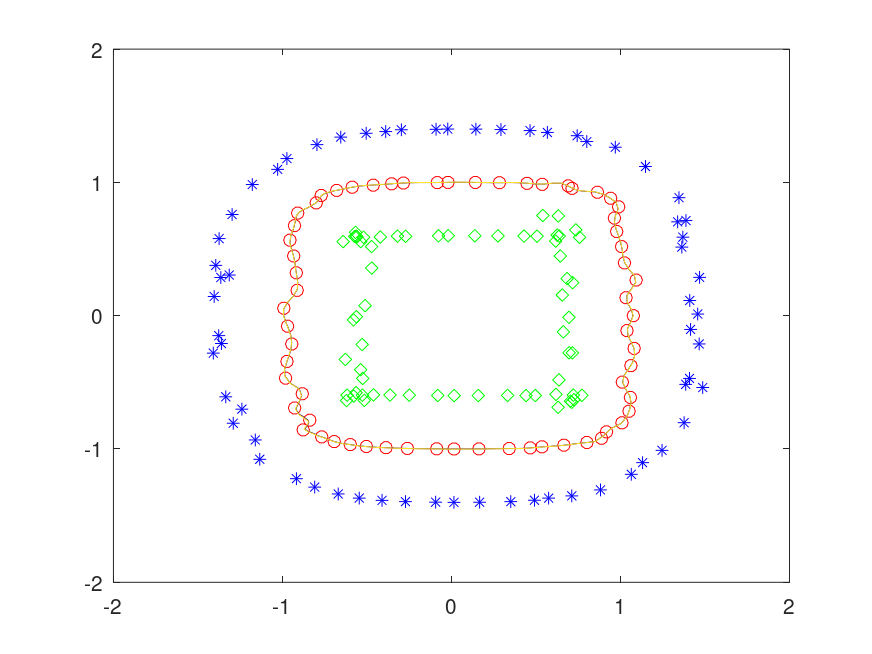
\includegraphics[width=0.6\textwidth]{problem_1iii.png}
    \caption{Feasible Region for minimizing $z = x_1 - 2x_2$}
    \label{fig:problem_1iii}
  \end{figure}
  \vfill
  \ \\
\end{solution}
  \pagebreak
  \item $(x_k)_{k \in \mathbb{N}}$, where $x_k = 3^{-k^2}$.

\begin{solution}
  \ \\
\end{solution}
  \pagebreak
\end{enumerate}